\section{Task 3}

\setcounter{task}{1}
\begin{frame}{Task 3}{Application control}
    \begin{tasknoinc}
        Consider the energy harvesting profile p(t) given in Figure 4 that repeats daily. What is the maximum average power $u_{max}$ that can be used by the system?
    \end{tasknoinc}
\end{frame}
\begin{frame}{Task 3}{Application control}
    \begin{solutionnoinc}
        \begin{figure}
            \centering
            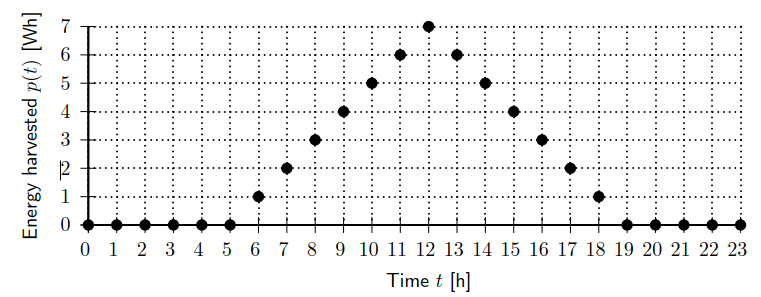
\includegraphics[scale=0.5]{figures/harvestingProfile.PNG}
        \end{figure}
    \end{solutionnoinc}
\end{frame}
\begin{frame}{Task 3}{Application control}
    \begin{solution}
        \begin{itemize}
            \item The daily harvested energy is calculated by: $(1Wh + 2Wh + 3Wh + 4Wh + 5H + 6Wh) * 2 + 7 Wh = 49Wh$
            \item This results in the following maximum average harvesting power: $u_{max} = \frac{49 Wh}{24h} = 2.04W$
        \end{itemize}
    \end{solution}
\end{frame}
\begin{frame}{Task 3}{Application control}
    \begin{tasknoinc}
        Given the knowledge of the daily energy input profile $p(t)$ in Figure 5, calculate the minimal battery size $B_{min}$ such that the used energy satisfies $u(t) = 2$ for every time interval during a day. Complete the diagram in Figure 6 with the daily evolution of the used energy $u(t)$ and the battery charge state $b(t)$ at the beginning of the interval for the found battery size $B_min$.
    \end{tasknoinc}
\end{frame}
\begin{frame}{Task 3}{Application control}
    \begin{solutionnoinc}
        \begin{itemize}
            \item The energy used during night, where the harvested energy is \alert{lower} than the consumed energy, is: $1Wh + 11 \cdot 2Wh + 1Wh = 24Wh$
            \item We need at least this much energy in our battery to compensate this deficit, meaning $B \geq 24Wh \Rightarrow B_{min} = 24Wh$.
        \end{itemize}
    \end{solutionnoinc}
\end{frame}
\begin{frame}{Task 3}{Application control}
\begin{figure}
    \centering
    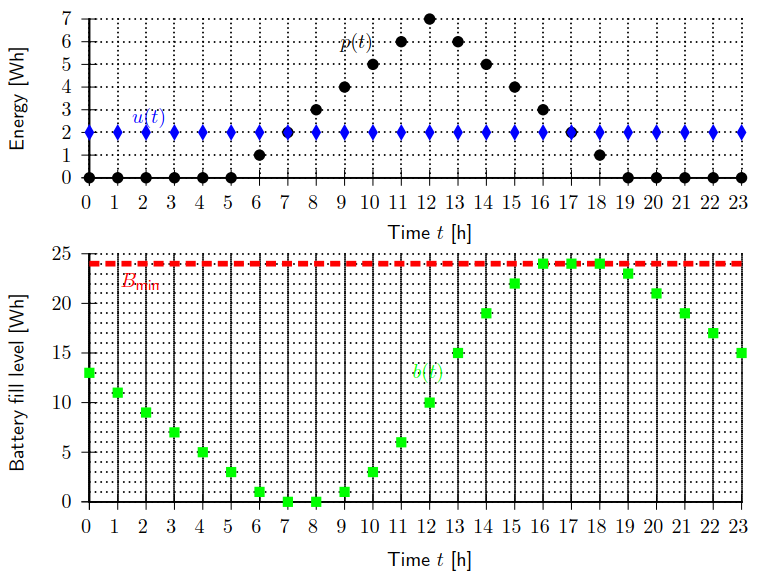
\includegraphics[scale=0.4]{figures/energyUsage.PNG}
\end{figure}
\end{frame}
